\section{Integrasi Sistem pada \emph{Real Robot}}
\label{sec:integrasirobot}

\begin{figure} [ht]
  \centering
  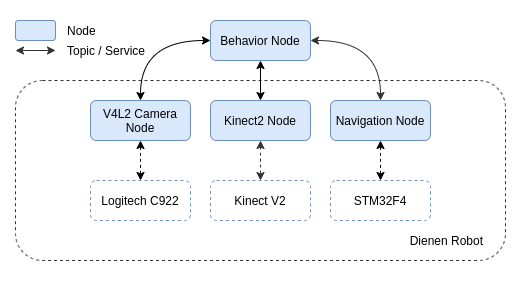
\includegraphics[scale=0.5]{gambar/integrasi-real-robot.png}
  \caption{Diagram integrasi sistem pada \emph{real robot}.}
  \label{fig:integrasirealrobot}
\end{figure}

Integrasi sistem pada \emph{real robot} dapat dilakukan dengan mengganti \emph{node} yang digunakan di simulasi dengan \emph{node} yang mengakses komponen yang ada pada \emph{real robot}.
Seperti yang terlihat pada gambar \ref{fig:integrasirealrobot},
  \emph{behavior node} yang digunakan masih sama,
  perbedaannya adalah digantinya \emph{camera plugin}, \emph{depth camera plugin}, dan \emph{navigation plugin} dengan \emph{V4L2 camera node}, \emph{Kinect2 node}, dan \emph{navigation node}.
Penggantian ini dapat dilakukan dengan mudah,
  karena seperti yang dijelaskan di bagian \ref{sec:behaviornode},
  \emph{behavior node} mengakses setiap \emph{node} yang mewakili komponen pada robot secara abstrak,
  yang mana keduanya dianggap \emph{node} yang sama oleh \emph{behavior node} terlepas dari bagaimana dan darimana data tersebut berasal,
  baik dari simulasi maupun dari \emph{real robot}.

\emph{V4L2 camera node} merupakan \emph{ROS 2 node} yang digunakan untuk mengakses kamera yang ada di sistem operasi \emph{Linux} dan mengirimkan data citra beserta informasi kamera melalui \emph{ROS 2 topic}.
\emph{Kinect2 node} merupakan \emph{ROS 2 node} yang digunakan untuk mengakses \emph{Kinect V2} menggunakan \emph{libfreenect2} dan mengirimkan data citra berwarna, citra kedalaman (\emph{depth image}), dan informasi kamera melalui \emph{ROS 2 topic}.
Sedangkan \emph{navigation node} adalah \emph{ROS 2 node} yang digunakan untuk mengakses \emph{STM32F4 controller} yang telah diprogram dengan sistem navigasi yang ada di robot \emph{Dienen}.
\emph{Navigation node} mengakses data yang ada di \emph{controller} tersebut menggunakan komunikasi UDP dan kemudian disalurkan oleh \emph{navigation node} melalui \emph{ROS 2 topic} sehingga bisa diakses oleh \emph{node} lain.

% \subimport{6-integrasi-robot}{1-navigation-node.tex}
% \subimport{6-integrasi-robot}{2-v4l2-camera-node.tex}
% \subimport{6-integrasi-robot}{3-kinect2-node.tex}
